\documentclass[twocolumn]{article}
\usepackage{graphicx} % Required for inserting images
\usepackage{newStyle}
\usepackage{titling}
\usepackage{stfloats}

\setlength{\droptitle}{-4em}

\title{RoSteALS Implementation and Robustness}
\author{Eugene Francisco}
\date{June 2026}

\begin{document}

\maketitle
\section*{Overview}
This writeup describes my implementation of Bui et al.'s\footnote{https://arxiv.org/pdf/2304.03400} RoSteALS technique for image watermarking. I include some deeper training details and some findings during training which the original paper did not discuss. My code can be found here.\footnote{https://github.com/EugeneFrancisco/ImageWatermarking}

As an overview of the technique, RoSteALS embeds watermarks into a cover image by using an image autoencoder and embedding information within the cover image's latent representation. More formally, let $E, G$ be an autoencoder. For a high fidelity image $c\in \R^{H\times W\times C}$, let $E(c) = z\in \R^{H'\times W'\times C}$ be $c$'s latent representation. For a latent variable $z\in \in \R^{H'\times W'\times C}$, let $G(z)\in \R^{H\times W\times C}$ be the generated image from the auto encoder.

How does RoSteALS watermark images? Let $c\in \R^{H\times W\times C}$ be an image we intend to watermark and $z = E(c)$ be its encoding. Let $s\in \R^\ell$ be a secret message we intend to embed in $c$. RoSteALS learns two neural networks:
\begin{enumerate}[label=(\roman*)]
\item First, it 	learns a message encoder $F_\theta$ which outputs $\delta = F_\theta(s) \in \R^{H' \times W'\times C}$. The watermarked latent is then $z + \delta$ and the watermarked image is $\tilde c = G(z + \delta)$.
\item Second, it leans a secret decoder $D_\varphi$ which outputs $\tilde s = D_\varphi(\tilde c)$, a reconstruction of the original message.
\end{enumerate}
The neural networks are parametrized by learnable parameters $\theta$ and $\varphi$. Note that the autoencoder $E, G$ is not learned and is fixed in advance. They are trained using two objectives:
\begin{enumerate}[label=(\alph*)]
\item $\L_{\mathrm{quality}} = \L_{\mathrm{LPIPS}}(\tilde c, c) + \alpha \Vert \gamma(\tilde c) - \gamma{c}\Vert_2^2$, where $\L_{\mathrm{LPIPS}}$ is the LPIPS image reconstruction loss and $\gamma$ is the mapping function from RGB to YUV.
\item $\L_{\mathrm{recovery}} = \mathrm{BCE}(s, \tilde s)$ where $\mathrm{BCE}$ is the binary cross entropy between $s$ and $\tilde s$.
\end{enumerate}
The training loss is then
\begin{align*}
	\L = \beta\L_{\mathrm{quality}} + \L_{\text{recovery}}.
\end{align*}

\section*{Implementation Details}
The \tc{purple}{purple} text corresponds to implementation details from \tc{purple}{Bui et al}. The \tc{olive}{olive} text corresponds to my own specific implementation details. \tc{purple}{The VQGAN vq-f4 autoencoder is used; this uses a latent dimension of $H' = H/4$ and $W' = W/4$. I fixed hyperparameters $\alpha = 1.5$ and $\beta$ is scaled dynamically (see below). I use the AdamW optimizer with learning rate $2\cdot 10^{-5}$.} \tc{olive}{I trained on the COCO training dataset from 2017 with $100{,}000$ images of size $256\times 256$ and a message length of $\ell = 50$.} \tc{purple}{I used curriculum learning to train with the following training schedule:}
\begin{enumerate}[label=(\alph*)]
\item \textit{Warmup phase 1}: \tc{purple}{ I fix $\beta = 0.1$ for the entirety of the phase and train $F_\theta$ and $D_\varphi$ until the bit accuracy reaches $0.9$.} \tc{olive}{Training is done with a fixed subset of $8$ randomly selected images from the total training set and a minibatch size of $4$.}\item \textit{Warmup phase 2:} \tc{olive}{I reveal an additional $50{,}000$ images. $\beta$ continues to be fixed at $0.1$. Batch size is bumped to $8$. This phase ends once bit accuracy reaches $0.8$.\footnote{In my experiments, the transition from \textit{warmup phase 1} to \textit{warmup phase 2} is typically followed by a drastic drop in bit accuracy, hence the lowered threshold.}}
\item \textit{Exposure phase 1: }\tc{olive}{Over the course of $5{,}000$\footnote{From my experiments, $5{,}000$ corresponded roughly to a $10$ percentage point increase in bit accuracy} training iterations,} \tc{purple}{I linearly increase $\beta$ from $0.1$ to $10$.}
\item \textit{Exposure phase 2:} \tc{olive}{I reveal the full $100{,}000$ image training set to the models. This phase ends once bit accuracy reaches $0.98$.}
\item \textit{Noising phase:} \tc{purple}{I insert a noising function $N$ between the creation of each watermarked image $\tilde c$ and message decoding. This means that the message decoder outputs $D(N(\tilde c))$.\footnote{Check Bui et al. for specifics on the noising functions used.}}
\end{enumerate}
For message encoder, I use the following Neural Network
\begin{verbatim}
    nn.Linear(50, 32*32*3), nn.SiLU,
    nn.Unflatten(1, (3, 32, 32)),
    nn.Upsample(scale_factor=2),
    nn.Conv2d(3, 3, 3, padding=1),
    nn.Conv2d(3, 3, 1)
\end{verbatim}
where \tc{purple}{the last convolution layer is $0$ initialized. The secret decoder is implemented as a ResNet-50 with the standard ImageNet head replaced by an MLP to $\R^{50}$ of logits representing the decoded message. I loaded ImageNet weights into the ResNet for training.} Training was done between an NVIDIA A10 and A100 GPU, with checkpoint (a) being trained with an A10 and the rest with A100s. Training took around 10 hours.
\begin{figure}
	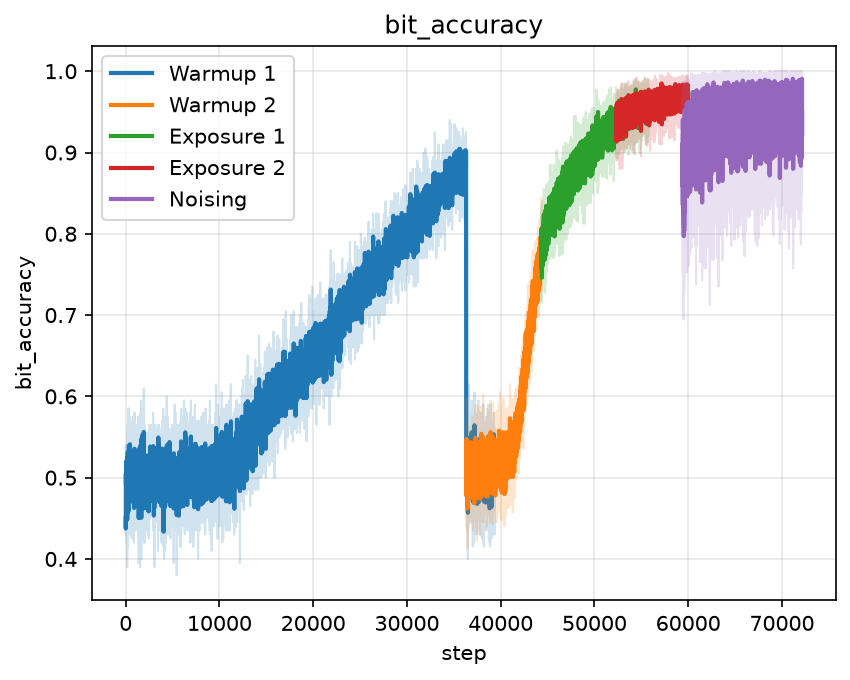
\includegraphics[scale=0.5]{images/bit_accuracy.png}\\
	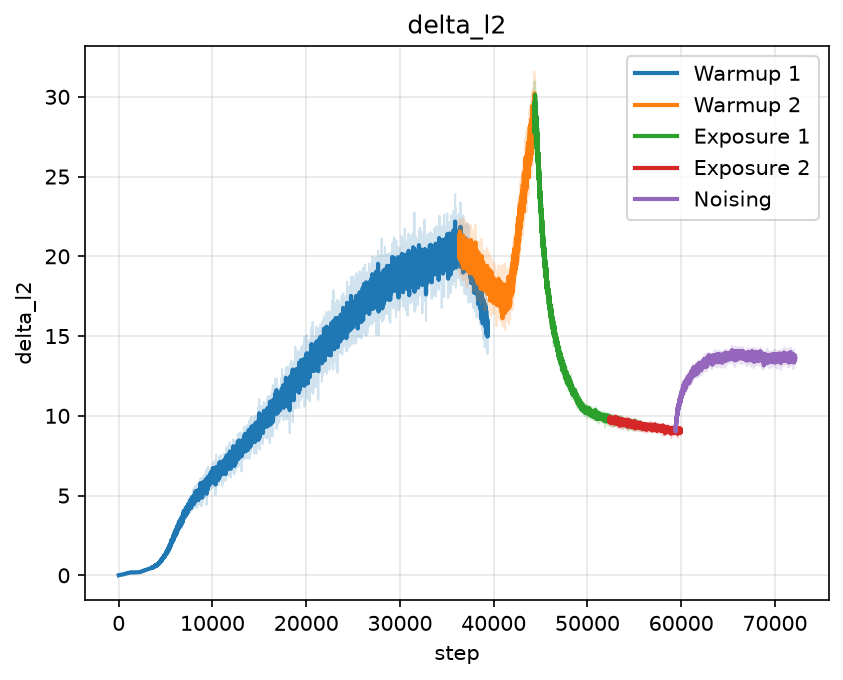
\includegraphics[scale=0.5]{images/delta_l2.png}\\
	\caption{\textit{top:} message recovery bit accuracy; \textit{bottom:} $\ell_2$ norm of the latent watermark $\delta$. Each color run is a separate training run restarted from a checkpoint of the previous runs. The overlap in runs (e.g., orange overlapping blue) is because some runs were allowed to run slightly longer after their checkpoint.}
	\label{fig:accuracy_norm}
\end{figure}
\section*{Discussion:}
The curriculum learning schedule described here exposes the model to only two mini-batches of data until bit-accuracy reaches $0.9$. This leads to significant overfitting and a sudden plummet in bit accuracy once a larger training set is revealed; however, my experiments suggest that this early training phase is critical.

In a separate experiment, I tried the same curriculum learning routine but revealing the model to $15{,}000$ training examples at the start instead of only $8$. In that trial, bit accuracy stagnated at around $15{,}000$ for the entire training run, revealing that overfitting on these minibatches is critical for training and perhaps allows the model to learn an encoding scheme to then apply to future images. This is possibly supported by Figure~\ref{fig:accuracy_norm} which shows how $\Vert \delta\Vert_2$ stays large when we begin exposing the model to more training examples.
\begin{figure}
	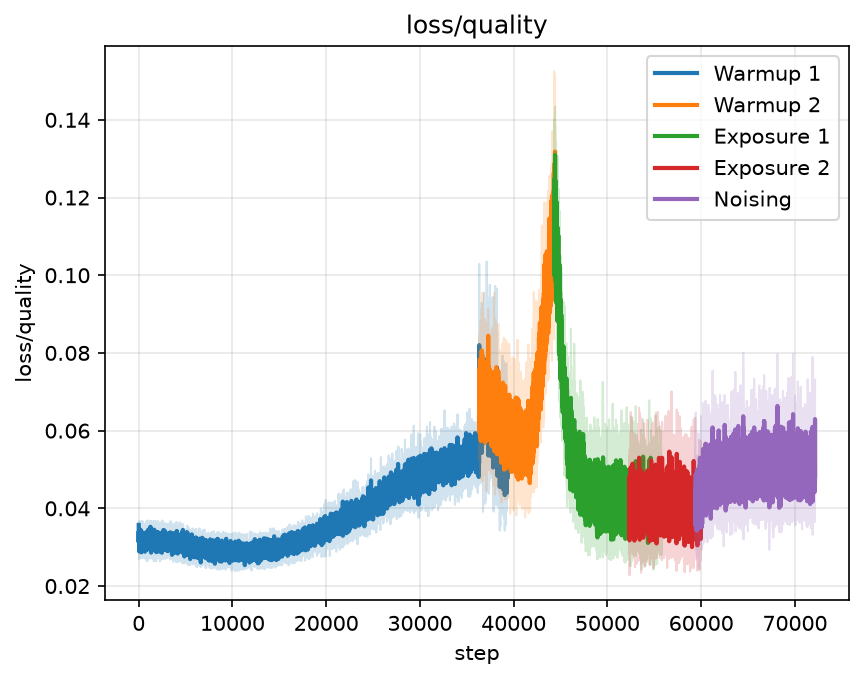
\includegraphics[scale=0.5]{images/loss_quality.png}\\
	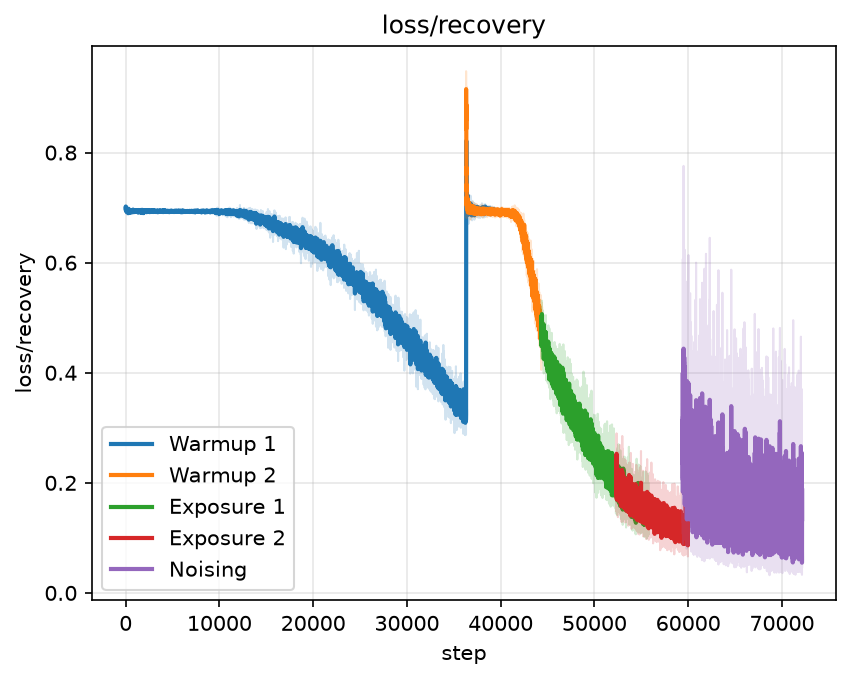
\includegraphics[scale=0.5]{images/loss_recovery.png}
	\caption{\textit{top:} $\L_{\mathrm{quality}}$; \textit{bottom:} $\L_{\mathrm{recovery}}$.}
\end{figure}
Because of this, it is possible that the choice of initial mini-batch can affect model robustness and quality which could allow for future work.

Loading the model with ImageNet weights was also critical to training; I tried a couple of training runs with randomly initialized Resnet50 weights to no avail.

\begin{figure*}
	
\includegraphics[scale=0.3]{images/zebra/cover.png}
	
\includegraphics[scale=0.3]{images/zebra/stego_warmup_1.png}
	
\includegraphics[scale=0.3]{images/zebra/stego_warmup_2.png}
	
\includegraphics[scale=0.3]{images/zebra/stego_exposure_2.png}
	
\includegraphics[scale=0.3]{images/zebra/stego_noising.png}
		
\includegraphics[scale=0.3]{images/train/cover.png}
	
\includegraphics[scale=0.3]{images/train/stego_warmup_1.png}
	
\includegraphics[scale=0.3]{images/train/stego_warmup_2.png}
	
\includegraphics[scale=0.3]{images/train/stego_exposure_2.png}
	
\includegraphics[scale=0.3]{images/train/stego_noising.png}
	
\includegraphics[scale=0.3]{images/messed_up_face/cover.png}
	
\includegraphics[scale=0.3]{images/messed_up_face/stego_warmup_1.png}
	
\includegraphics[scale=0.3]{images/messed_up_face/stego_warmup_2.png}
	
\includegraphics[scale=0.3]{images/messed_up_face/stego_exposure_2.png}
	
\includegraphics[scale=0.3]{images/messed_up_face/stego_noising.png}
	
\includegraphics[scale=0.3]{images/big_face/cover.png}
	
\includegraphics[scale=0.3]{images/big_face/stego_warmup_1.png}
	
\includegraphics[scale=0.3]{images/big_face/stego_warmup_2.png}
	
\includegraphics[scale=0.3]{images/big_face/stego_exposure_2.png}
	
\includegraphics[scale=0.3]{images/big_face/stego_noising.png}
	
\includegraphics[scale=0.3]{images/menu/cover.png}
	
\includegraphics[scale=0.3]{images/menu/stego_warmup_1.png}
	
\includegraphics[scale=0.3]{images/menu/stego_warmup_2.png}
	
\includegraphics[scale=0.3]{images/menu/stego_exposure_2.png}
	
\includegraphics[scale=0.3]{images/menu/stego_noising.png}
	\caption{Sample images from training.}
		\label{fig:images}
\end{figure*}


After inserting noise, there is a clear compromise with image quality that is made as can be seen in Figure~\ref{fig:images}. In Bui et al's paper, the post-noising watermarks are much less obvious which I attribute to more training time post-noising. However, the \textit{Exposure 2} watermarks are almost invisible with a few notable failure cases.

All watermarking models struggle with human faces and with text (see bottom Figure~\ref{fig:images}). These defects essentially disappear for faces and are slightly alleviated for text once these subjects are larger in the image, suggested that these watermarks fare best with higher resolutions (Figure~\ref{fig:images} row 4 and 5).

Bit accuracy and quality loss across different transformations applied to the COCO test set from 2017 is below.
\begin{table}[h]
\centering
\begin{tabular}{lc}
\hline
Metric & Value \\
\hline
Quality Loss & 0.050 \\
\hline
\multicolumn{2}{l}{\textit{Bit Accuracy}} \\
\hline
Identity & 0.996 \\
Differentiable & 0.985 \\
Gaussian Noise & 0.886 \\
Shot Noise & 0.894 \\
Impulse Noise & 0.877 \\
Defocus Blur & 0.986 \\
Fog & 0.991 \\
Brightness & 0.992 \\
Contrast & 0.978 \\
Elastic Transform & 0.730 \\
Pixelate & 0.995 \\
JPEG Compression & 0.837 \\
Speckle Noise & 0.924 \\
Gaussian Blur & 0.987 \\
Spatter & 0.988 \\
Saturate & 0.986 \\
\hline
\end{tabular}
\caption{Test results for Experiment 1.}
\label{tab:experiment_1}
\end{table}















\section*{}

\end{document}